\documentclass{article}
\PassOptionsToPackage{numbers,sort&compress}{natbib}
\usepackage[preprint]{../proposal/neurips_2026}
\usepackage[utf8]{inputenc}
\usepackage[T1]{fontenc}
\usepackage{amsmath}
\usepackage{booktabs}
\usepackage{float}
\usepackage{graphicx}
\usepackage{microtype}
\usepackage[hidelinks]{hyperref}

\title{Selecting Image-Editing Recipes Before Rendering:\\A Small-Data Study of Preference and Computation}
\author{Lin Zihan\\HKUST(GZ)\\Student ID: 50027371}

\begin{document}
\maketitle

\begin{abstract}
Rendering several edits of one image can be expensive. I study whether a model can select an editing recipe before rendering and how much image features contribute to that decision. I labeled 1,145 outputs from 100 COCO sources. I compare selectors using source features, output features, and recipe descriptors through five-fold evaluation grouped by source. The pre-render selector makes 67/100 correct decisions, compared with 70/100 for a post-render scorer, 62/100 for a recipe baseline, and 60/100 for a fixed candidate position. Correct decisions select an acceptable output or reject a source whose outputs are all unacceptable. All four policies make zero correct rejections. The pre-render selector agrees with the recipe baseline on 87 sources. Shuffling source features lowers its mean success to 65.8/100. These results show a small acceptability gap between pre- and post-render selection, with a modest contribution from image features. Historical generation logs suggest potential compute savings; deployment timing remains to be measured.
\end{abstract}

\section{Introduction}
Styling, material reconstruction, and composition provide many ways to edit a photograph. An editor can render several recipes and rank their outputs. Selecting a recipe \emph{before} rendering could reduce this work. I ask two questions: how closely can pre-render selection match the quality of post-render selection, and how much do image features add to preferences learned across recipes?

I study these questions using a candidate bank I labeled. I count a decision as correct if the selector chooses an acceptable output or rejects a source with no acceptable outputs. For sources with at least one acceptable output, I also report how often the selector chooses my top-ranked edit. A recipe baseline learns preferences for operation sequences, references, and strengths across sources. I compare it with models that also receive image features. The evaluation covers recipes that completed generation, so its conclusions concern selection within this recorded bank.

\section{Related Work}
NIMA predicts the distribution of aesthetic ratings for an image \citep{talebi2018nima}. Ren et al.~\citep{ren2017personalized} model how an individual's ratings differ from generic aesthetic scores. I use my rankings of edits to the same image to study whether a selector can identify a preferred edit before rendering it. CLIP supplies frozen image embeddings \citep{radford2021clip}. SAM 2, InstantStyle, and DragonDiffusion supply pretrained editing components \citep{ravi2024sam2,wang2024instantstyle,mou2024dragondiffusion}. I train a selector to choose an operation sequence and reference before rendering its output.

\section{Method}
\paragraph{Candidates and feedback.} I use 100 COCO val2017 images, ten from each of ten categories \citep{lin2014coco}. These sources are separate from the 20 pilot images used in recipe design. Each source has 12 candidate recipes containing one to three operations: color adjustment, composition, collage, styling, material reconstruction, or object movement. The first 60 sources use automatic SAM 2 subject selection; the remaining 40 use detector-box prompts for whole objects. Style and material references stay fixed during learning. Of 1,200 attempts, 1,145 complete generation. I was the sole annotator. For each source, I ranked the outputs I deemed acceptable and labeled the other completed outputs as unacceptable. This yields 372 acceptable outputs and four sources whose outputs are all unacceptable. Aesthetic evaluation covers the completed outputs.

\paragraph{Representations.} Frozen CLIP encodes the source and its masked subject on a white background into two 1,024-dimensional vectors. A missing mask gives a zero subject vector. The post-render scorer also encodes the output. A 131-dimensional descriptor represents the ordered operations, reference IDs, strengths, and estimated subject count. Pre- and post-render inputs have 2,179 and 3,203 dimensions. The recipe baseline uses the post-render input layout with all image embeddings set to zero. It retains subject count and the recipes proposed for each source, so it measures the value of CLIP features beyond this context. Each model has two hidden layers of 64 and 32 units with ReLU activations, dropout $0.25$ after the first layer, and two outputs: preference score $r$ and acceptability logit $a$.

\paragraph{Training and decision.} Let $S$ be the training sources, $C_s$ the completed candidates for source $s$, and $P_s$ its decisive preference pairs. These pairs compare two ranked outputs or an acceptable output with an unacceptable one. Let $S_P$ contain sources with at least one such pair. With $(i,j)$ ordered so that $i$ is preferred, and acceptability label $y_i\in\{0,1\}$, the objective is
\begin{equation}
\begin{aligned}
\mathcal{L}={}&\frac{1}{|S_P|}\sum_{s\in S_P}\frac{1}{|P_s|}
\sum_{(i,j)\in P_s}\operatorname{BCELogits}(r_i-r_j,1)\\
&+\frac{1}{|S|}\sum_{s\in S}\frac{1}{|C_s|}
\sum_{i\in C_s}\operatorname{BCELogits}_{w_+}(a_i,y_i).
\end{aligned}
\end{equation}
The two losses receive equal weight, and each averages contributions by source. The positive-class weight $w_+$ is the training-fold negative-to-positive ratio, with a minimum of one. AdamW uses learning rate $3\times10^{-4}$ and weight decay $0.05$. Training runs on CPU for 80 full-batch epochs, reusing each candidate's score across pairs within an epoch. The selector chooses the recipe with the highest $r$ among those with $a>t$, or rejects the source when this set is empty. The threshold $t$ is selected within the training fold.

\section{Experimental Design}
Five folds each hold out two sources per category, giving 20 evaluation sources and 80 training sources. All recipes from one source stay in the same fold. Within the training set, a 60/20 split selects $t$ from ten thresholds using source-level success. The model is then trained afresh on all 80 sources. Each fit uses 80 epochs, with one seed per fold. Success means choosing an acceptable output or correctly rejecting a source whose outputs are all unacceptable. I also count first-choice hits, unacceptable selections, and false rejections of sources that contain an acceptable output.

All policies use the same outer folds and completed candidates. The fixed-position baseline selects a candidate position using training labels; the recipe at that position varies by source. The recipe baseline supplies a learned comparison using descriptors and subject count. The post-render model supplies a learned scorer with access to the generated output. The pre-render model uses source features and recipe descriptors. The evaluation script, recorded results, threshold settings, and reproduction instructions are available in the project repository (\url{https://github.com/Zl-Hhhhhh/DL_project}).

\section{Results and Discussion}

\begin{table}[H]
\centering
\caption{Five-fold development results (100 sources; top-choice hits among 96 sources with an acceptable output). The selected position is c06 in every training fold.}
\label{tab:results}
\small
\begin{tabular}{lrrrr}
\toprule
Policy & Correct / 100 & Top choice / 96 & Bad choices & False rejects \\
\midrule
Fixed position & 60 & 19 & 40 & 0 \\
Recipe baseline & 62 & 19 & 38 & 0 \\
Pre-render MLP & 67 & 18 & 32 & 1 \\
Post-render MLP & 70 & 21 & 30 & 0 \\
\bottomrule
\end{tabular}
\end{table}

\begin{figure}[H]
\centering
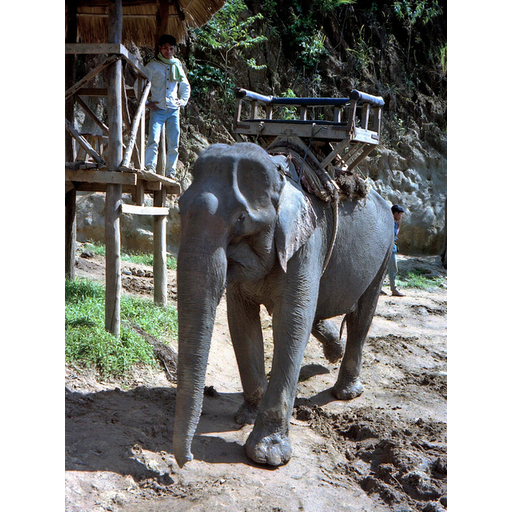
\includegraphics[width=.31\linewidth]{figures/coco_158945_source.png}\hfill
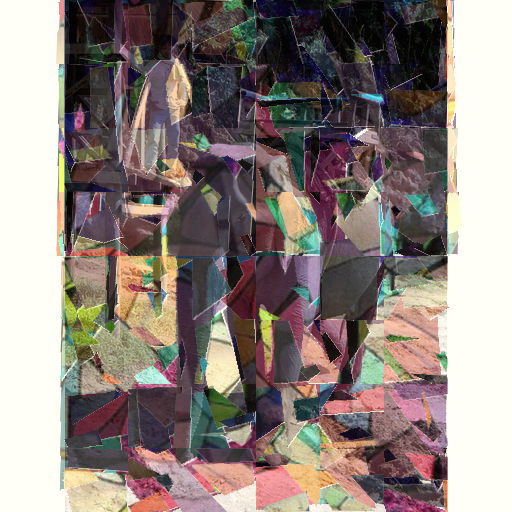
\includegraphics[width=.31\linewidth]{figures/coco_158945_pre_render.png}\hfill
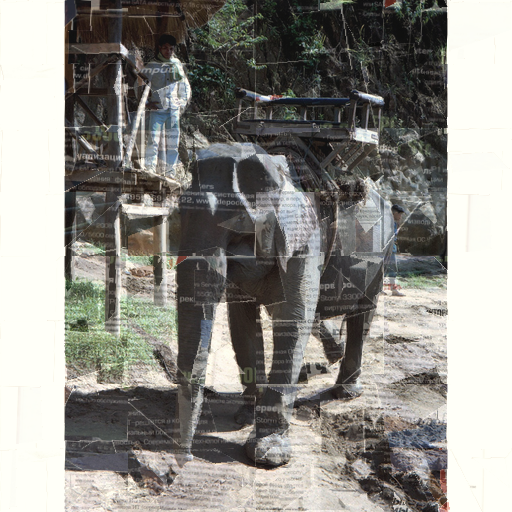
\includegraphics[width=.31\linewidth]{figures/coco_158945_recipe_baseline.png}
\caption{An example of differing selections (COCO 158945). From left to right, the panels show the source, the pre-render selection c05 (which I labeled acceptable), and the recipe-baseline selection c06 (which I labeled unacceptable). Both apply material reconstruction then warm-film adjustment, using stained glass and newspaper references, respectively.}
\label{fig:example}
\end{figure}

Pre-render selection reaches 67/100 correct decisions, three fewer than post-render selection (Table~\ref{tab:results}). The recipe baseline reaches 62/100, and the fixed position reaches 60/100. The pre-render model and recipe baseline make the same choice on 87 sources. The pre-render model succeeds where the baseline fails on six sources; the reverse occurs on one. Figure~\ref{fig:example} shows one of these cases.

To probe dependence on image features, I shuffle the paired source and subject embeddings among sources within each evaluation fold. Recipe descriptors, model weights, and thresholds stay fixed. Across 30 permutations, success averages 65.8/100 (range 62--68), a decrease of 1.2 decisions. These repeats measure sensitivity to shuffled inputs. Together with the agreement between models, they suggest that recipe descriptors explain much of the observed selection behavior. The added contribution of CLIP features appears modest on this bank.

Rejection remains a weakness: all four policies select unacceptable outputs for the four entirely unacceptable sources. Inner threshold selection chooses zero in every pre- and post-render fold. The pre-render model also rejects one source that contains an acceptable output. Its first-choice hit rate is 18/96, compared with 21/96 after rendering. Thus the acceptability counts are close, while matching my top-ranked output remains difficult for both models.

The 1,200 generation attempts total 27,393 recorded seconds, or 274 seconds per source on the local NPU pipeline. The fixed-position baseline selected 100 candidates totaling 2,986 recorded seconds and made 60 correct decisions. The pre-render selector chose 99 candidates totaling 2,992 recorded seconds, rejected one source, and made 67 correct decisions. At these different coverage levels, the selected candidates had similar total recorded generation times, and the learned selector made seven more correct decisions. Deployment timing must include feature extraction, retries, and the effects of subject routing and caches. The evaluation gives selectors advance knowledge of which recipes completed generation by filtering out 55 failures. This makes the cost comparison optimistic for deployment.

\newpage
These 100 sources informed method and loss development, so the results are development estimates. Each fold uses one seed, and the labels reflect only my preferences. The two subject-selection procedures also introduce variation across the bank. A stronger evaluation would use fresh sources, several training seeds, and additional annotators. Running the full editing pipeline would test segmentation quality, rejection, generation failures, and the quality achieved for a given time budget.

\section{Conclusion}
On this development bank, pre-render selection achieves 67 correct decisions compared with 70 after rendering. Its agreement with the recipe baseline and its response to feature shuffling suggest a modest contribution from image embeddings. The results motivate selecting recipes before generation. Fresh evaluation images and a timed pipeline are the next steps for measuring generalization and compute savings.

\begin{thebibliography}{8}
\bibitem{talebi2018nima} H. Talebi and P. Milanfar. NIMA: Neural Image Assessment. \emph{IEEE Transactions on Image Processing}, 2018. \url{https://arxiv.org/abs/1709.05424}.
\bibitem{ren2017personalized} J. Ren et al. Personalized Image Aesthetics. \emph{ICCV}, 2017. \href{https://openaccess.thecvf.com/content_iccv_2017/html/Ren_Personalized_Image_Aesthetics_ICCV_2017_paper.html}{CVF Open Access}.
\bibitem{radford2021clip} A. Radford et al. Learning Transferable Visual Models From Natural Language Supervision. \emph{ICML}, 2021. \url{https://arxiv.org/abs/2103.00020}.
\bibitem{ravi2024sam2} N. Ravi et al. SAM 2: Segment Anything in Images and Videos. \emph{ICLR}, 2025. \url{https://arxiv.org/abs/2408.00714}.
\bibitem{wang2024instantstyle} H. Wang et al. InstantStyle: Free Lunch towards Style-Preserving in Text-to-Image Generation. \emph{arXiv:2404.02733}, 2024. \url{https://arxiv.org/abs/2404.02733}.
\bibitem{mou2024dragondiffusion} C. Mou et al. DragonDiffusion: Enabling Drag-style Manipulation on Diffusion Models. \emph{ICLR}, 2024. \url{https://arxiv.org/abs/2307.02421}.
\bibitem{lin2014coco} T.-Y. Lin et al. Microsoft COCO: Common Objects in Context. \emph{ECCV}, 2014. \url{https://arxiv.org/abs/1405.0312}.
\end{thebibliography}
\end{document}
